%----------------------------------------------------------------------------------------
%	PACKAGES AND THEMES
%----------------------------------------------------------------------------------------
\documentclass[aspectratio=169,xcolor=dvipsnames]{beamer}
\usetheme{Simple}
\usepackage{hyperref}
\usepackage{graphicx} % Allows including images
\usepackage{booktabs} % Allows the use of \toprule, \midrule and \bottomrule in tables
\usepackage{graphicx}
\setbeamertemplate{caption}[numbered]
\setbeamertemplate{footline}[text line]{%
  \parbox{\linewidth}{\vspace*{-8pt}Github Repository: \href{https://github.com/sanjay-kv/Semi-supervised-sequence-learning-Project}{https://github.com/sanjay-kv/Semi-supervised-sequence-learning-Project}.\hfill\insertpagenumber}}
\setbeamertemplate{navigation symbols}{}

%----------------------------------------------------------------------------------------
%	TITLE PAGE
%----------------------------------------------------------------------------------------

% The title
\title[short title]{Project Final Presentation}
\subtitle{Semi-supervised Sequence Learning}

\author[Sanjay K V] {Sabiha Sultana\inst{1}, Piyakorn Munegan\inst{2},\\ 
Sanjay Kanakkot Viswanathan\inst{3},\break Mohammed Rizwan Amanullah\inst{4}}
\institute[NTU] % Your institution may be shorthand to save space
{
    % Your institution for the title page
    Department of Computing, \\
    Macquarie University 
    \vskip 3pt
}
\date{\today} % Date, can be changed to a custom date


%----------------------------------------------------------------------------------------
%	PRESENTATION SLIDES - Make Presentation title and source in 1st page, put earlier suggestion to consideration as example. no justification of paper again. Look at the email suggestion about predicting performance.
%----------------------------------------------------------------------------------------

\begin{document}

\begin{frame}
    % Print the title page as the first slide
    \titlepage
\end{frame}

\begin{frame}{Recap - Semi-supervised Sequence Learning Project}
    % Throughout your presentation, if you choose to use \section{} and \subsection{} commands, these will automatically be printed on this slide as an overview of your presentation
    \tableofcontents
%------------------------------------------------
%Recap
%------------------------------------------------
\begin{itemize}
        \item Goal: Replicating project which aims on unlabelled data to improve sequence learning with Recurrent network 
        \item (LM-LSTM) Language modelling. Predict what comes next in sequence. 
        \item (SA-LSTM) Reads input sequence into vectors and predict the input sequence again. 
         \item \alert {Requirements:} AWS(EC2) with Python 3, tensorflow v 1.15.5
     \item \alert{Source:} \href{https://arxiv.org/pdf/1511.01432v1.pdf}{https://arxiv.org/pdf/1511.01432v1.pdf}
    \item \alert{Source Repo:}\href{ https://github.com/tensorflow/models/tree/master/research/adversarial_text}{ https://github.com/tensorflow/models/tree/master/research/adversarial}
    \item Dataset: \break
            - IMDB movie review dataset\break     
            - DBpedia dataset (DBpedia abstracts and its categories)
 
    \end{itemize}

\end{frame}

%------------------------------------------------
%Replication2
%------------------------------------------------

\begin{frame}{Recap - Replication Process}
    \begin{itemize}
    \newline
    \newline
         \begin{figure}
            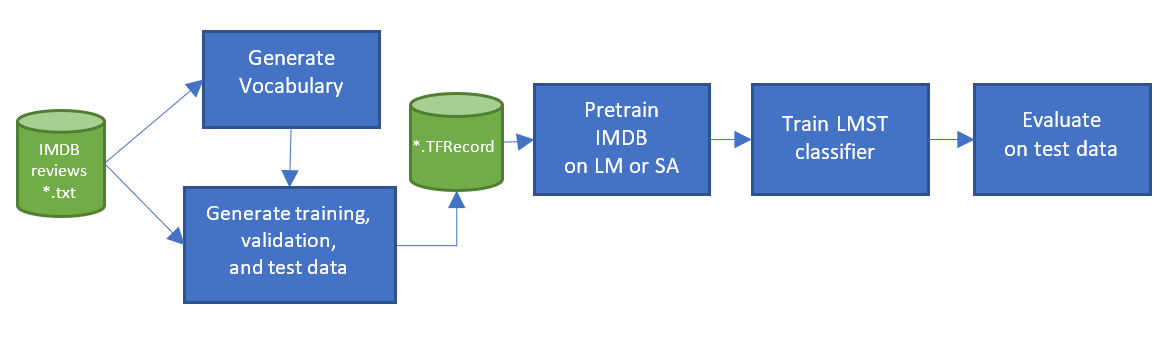
\includegraphics[width=400]{replicationFlow2.PNG}
               \caption{Explains the flow of replication for Sentiment Analysis.}
        \end{figure}
        \newline
        \newline
         \break
    \end{itemize}
\end{frame}

%------------------------------------------------

%------------------------------------------------
% Sanjay Issues Explanation in details
%------------------------------------------------
\begin{frame}{IMDB - Data Generation}
    % Throughout your presentation, if you choose to use \section{} and \subsection{} commands, these will automatically be printed on this slide as an overview of your presentation
    \tableofcontents
%------------------------------------------------
%Overview
%------------------------------------------------

    \begin{columns}[c] % The "c" option specifies centered vertical alignment while the "t" option is used for top vertical alignment

        \column{.45\textwidth} % Left column and width
        \textbf{The Process}
        \begin{enumerate}
            \item Created Python Script.
            \item Scrapped the data in 7 categories.
            \item BeautifulSoup python package.
        \end{enumerate}

        \column{.5\textwidth} % Right column and width
         Used python script to scrap the recent reviews from IMDB Website. Scrapped 15\% of original data-set, latter manually annotated 2000 file, among them as positive and negative sentiment category and 1000 treated as unlabelled data.

    \end{columns}   \\
    
\begin{table}[h!]
  \begin{center}
    \caption{A summary of total data scrapped using Beautifulsoup from IMDB Website.}
    \label{tab:table1}
    \begin{tabular}{|l|c|r|} % <-- Alignments: 1st column left, 2nd middle and 3rd right, with vertical lines in between
      \hline
      \textbf{Dataset } & \textbf{Labelled} & \textbf{Unlabelled}\\
      
      \hline
      IMDB & 2000 & 1000 \\
      \hline
     
    \end{tabular}
  \end{center}
\end{table}   \newline
\begin{itemize}
      
    \item \alert{Repository:}\href{ https://github.com/sanjay-kv/Semi-supervised-sequence-learning-Project/tree/main/imdb_review_scrapping}{ https://github.com/sanjay-kv/Semi-supervised-sequence-learning-Project/tree/main/imdb-review-scrapping}
 
    \end{itemize}
\end{frame}
%------------------------------------------------

%------------------------------------------------
%justification of original work
%------------------------------------------------

\begin{frame}{Amazon New Data Generation}
    \begin{itemize}
        \item Scrapped amazon.in website using selenium.
        \item We have extracted product listing and product information for ten categories. \break 
            - After extraction, we are manually tagging the product listing. \break
    \end{itemize}
    
          \begin{table}[h!]
  \begin{center}
    \caption{A summary of total data scrapped using Beautifulsoup from IMDB Website.}
    \label{tab:table1}
    \begin{tabular}{|l|c|} % <-- Alignments: 1st column left, 2nd middle and 3rd right, with vertical lines in between
      \hline
      \textbf{Dataset } & \textbf{Scrapped Listings} \\
      
      \hline
      Amazon & 3154  \\
      \hline
     
    \end{tabular}
  \end{center}
\end{table}
\begin{itemize}
      
    \item \alert{Repository:}\href{ https://github.com/sanjay-kv/Semi-supervised-sequence-learning-Project/tree/main/amazon_scrapping}{ https://github.com/sanjay-kv/Semi-supervised-sequence-learning-Project/tree/main/amazon-scrapping}
 
    \end{itemize}
\end{frame}


%----------------------------------------------------------------------------------------


%------------------------------------------------
% Dataset for the sentiment classification task}
%------------------------------------------------
\begin{frame}{Dataset for the sentiment classification task}
    \tableofcontents

    \textbf{Dataset}
    \begin{enumerate}
        \item Original IMDB  movie review dataset.\break 
            - Training set: 25,000 labeled and 50,000 unlabeled reviews.\break 
            - Test set: 25,000 labeled reviews.\break
            
         \item  Replication of 5\% the size of the original IMDB dataset.\break 
            - Training set: 1,111 labeled and 1,111 unlabeled reviews.\break 
            - Test set: 1,111 labeled reviews.\break
            
        \item Replication of new IMDB dataset.\break 
            - Training set: 1,000 labeled and 1,000 unlabeled reviews.\break 
            - Test set: 1,000 labeled reviews.\break
        \end{enumerate}
\end{frame}
%------------------------------------------------

%------------------------------------------------
% Dataset for the product classification task}
%------------------------------------------------
\begin{frame}{Dataset for the product classification task}
    \tableofcontents

    \textbf{Dataset}
        \begin{enumerate}
        \item Dataset: DBpedia dataset.\break 
            - Training set: 560,000 labeled examples.\break
            - Test set: 70,000 examples.\break
         
         \item Replication of 2\% the size of the original DBpedia dataset.\break 
            - Training set: 11,200 labeled examples.\break 
            - Test set: 1,400 examples.\break
        
        \item Replication of new Amazon dataset\break 
            - Training set: 2,795 examples.\break 
            - Test set: 395 examples.\break
        \end{enumerate}
\end{frame}
%------------------------------------------------
%-------------------------------------------------------------

%------------------------------------------------
% Sanjay Issues Explanation in details
%------------------------------------------------
\begin{frame}{Pre-training Process}
    % Throughout your presentation, if you choose to use \section{} and \subsection{} commands, these will automatically be printed on this slide as an overview of your presentation
    \tableofcontents
%------------------------------------------------
%Hyperparameters tuning
%------------------------------------------------

 %Adding picture

  \begin{figure}
   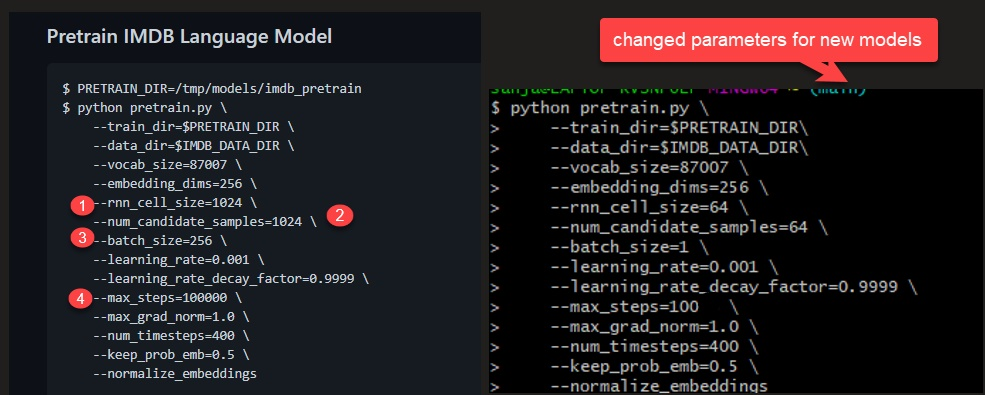
\includegraphics[width=420]{updated_model_1.jpg}
      \caption{On left the Default parameter, On right Parameters we used for replication}
\end{figure}

\end{frame}
%----

%------------------------------------------------
\begin{frame}{Evaluation Results}
    % Throughout your presentation, if you choose to use \section{} and \subsection{} commands, these will automatically be printed on this slide as an overview of your presentation
    \tableofcontents
%------------------------------------------------
%Overview
%------------------------------------------------

\begin{table}[h!]
    \begin{center}
    
    \caption{Summary of the accuracy scores of models on the IMDB sentiment classification task}
    \label{tab:table1}
    \begin{tabular}{|l|r|r|r|} % <-- Alignments: 1st column left, 2nd middle and 3rd right, with vertical lines in between
      \hline
      \textbf{Dataset} & \textbf{LM-LSTM} & \textbf{SA-LSTM} & \textbf{LSTM} \\
      \hline
      Original IMDB dataset (original work) & 92.36 & 92.76 & 86.5 \\
      5 \% of the original IMDB dataset & 57.6 & 56.8 & - \\
      New IMDB dataset & 50 & 50 & 50 \\
      \hline
    \end{tabular}
    
    \caption{Summary of the accuracy scores of models on the product classification task}
    \label{tab:table2}
    \begin{tabular}{|l|r|r|r|r|} 
      \hline
      \textbf{Dataset} & \textbf{LM-LSTM} & \textbf{SA-LSTM} & \textbf{LSTM} & \textbf{SVM}\\
      \hline
      Original DBpedia dataset (original work) & 98.5 & 97.66 & 86.36 & -\\
      2 \% of the original DBpedia dataset & 7.1 & 7.1 & 7.1 & - \\
      New Amazon dataset & 9.4 & 9.4 & 9.4 & 4.54\\
      \hline
    \end{tabular}
    \break
    \break
    \footnotesize{Pretraining: LM =  Language Model, and SA = Sequence Autoencoder}
  \end{center}
\end{table}

\end{frame}
%------------------------------------------------


%------------------------------------------------
% Findings and conclusion for the project
%------------------------------------------------
\begin{frame}{Findings/ Conclusion}
    \tableofcontents
%------------------------------------------------
%Overview
%------------------------------------------------

    \begin{columns}[c] % The "c" option specifies centered vertical alignment while the "t" option is used for top vertical alignment

        \column{.45\textwidth} % Left column and width
        \textbf{The Process}
        \begin{enumerate}
            \item In sentiment Analysis we were able to replicate and validate the accuracy.
            \item Impact of less data has been observed in the obtained accuracy of the classification task of amazon dataset
        \end{enumerate}

        \column{.5\textwidth} % Right column and width
         We Ensured for NLP task can use LSTM recurrent network, along with it the team were able to find and validate sequence auto-encoder can stabilize the LSTM learning process. LSTM Outperformed all other evaluation categories.

    \end{columns}   \\

\end{frame}
%------------------------------------------------

%----------------------------------------------------------------------------------------
\begin{frame}
    \Huge{\centerline{The End}}
\end{frame}

%----------------------------------------------------------------------------------------

\end{document}